\documentclass{article}
\usepackage{graphicx}
\usepackage{amsmath,amsthm} 
\usepackage{amsfonts} 
\usepackage{pdfpages}

\begin{document}

\title{COMP3331 Lab1}
\author{Ruofei HUANG}

\maketitle

\section{Exercise 1}

\subsection{}
129.94.242.2
More than one output is for DNS side of load balancing.

\subsection{}
localhost
All the connection to this device is actual to current computer. Every connection go through this address will go through a hardware loopback to this device.

\section{Exercise 2}

\subsection{Ping Reachability}

\begin{tabular}{|c|c|l|}
    \hline
    Reachable& Hostname &Reason \\ 
    \hline
    No &www.cse.unsw.edu.au    &Host IP is setted to not\\
    && answering the ping request.\\
    \hline
    No &www.getfittest.com.au  &No result from dns.\\
    \hline
    Yes&www.mit.edu&\\
    \hline
    Yes&www.intel.com.au&\\
    \hline
    Yes&www.tpg.com.au&\\
    \hline
    No &www.hola.hp            &Invalid domain name.\\
    \hline
    Yes&www.amazon.com&\\
    \hline
    Yes&www.tsinghua.edu.cn&\\
    \hline
    No &www.kremlin.ru         &Host doesn't answer the request.\\
    \hline
    Yes &8.8.8.8&\\
    \hline
\end{tabular}

\subsection{Ping Unreachable Host, Test by Browser}
\begin{tabular}{|c|c|}
    \hline
    Hostname & Web Reachable\\
    \hline
    www.cse.unsw.edu.au   &Yes \\
    www.getfittest.com.au &No \\
    www.hola.hp           &No \\
    www.kremlin.ru        &Yes \\
    \hline
\end{tabular}

\section{Exercise 3}
\subsection{}
21 routers.\\
3rd and 4th router \\

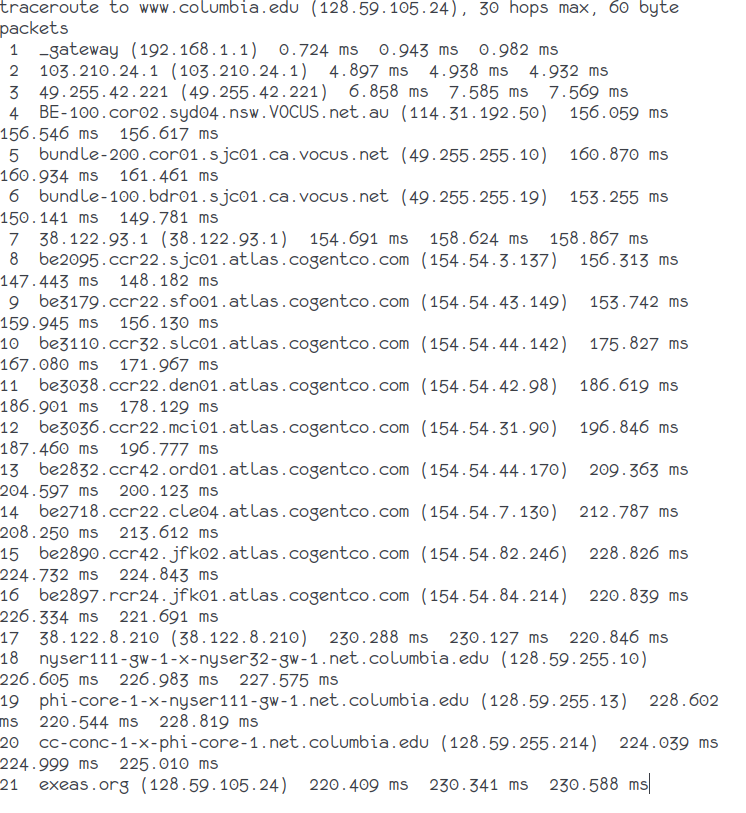
\includegraphics[width=\textwidth]{img/tr_columbia.png}

\subsection{}
Diverage at 49.255.42.221\\
Or Diverage from a router group? BE-100.cor02.syd04.nsw.VOCUS.net.au \\
49.255.42.221 is belong to VOCUS PTY LTD\\
BE-100.cor02.syd04.nsw.VOCUS.net.au is belong to Vocus Communications Ltd\\

Both routers are belong to vocus Communications which is a ISP for small ISP, in my point of view. They're business is target to datacenter, ISP, etc. And they have national wide optical caples and cable go aboard.

I couldn't find out the geological location about both network.

No, Uk is further than japan but I observed less hops in www.lancaster.ac.uk
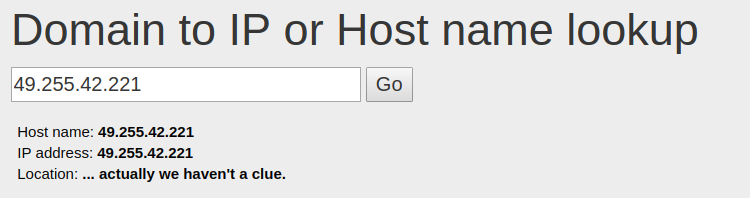
\includegraphics[width=\textwidth]{Location_wont_work.png}
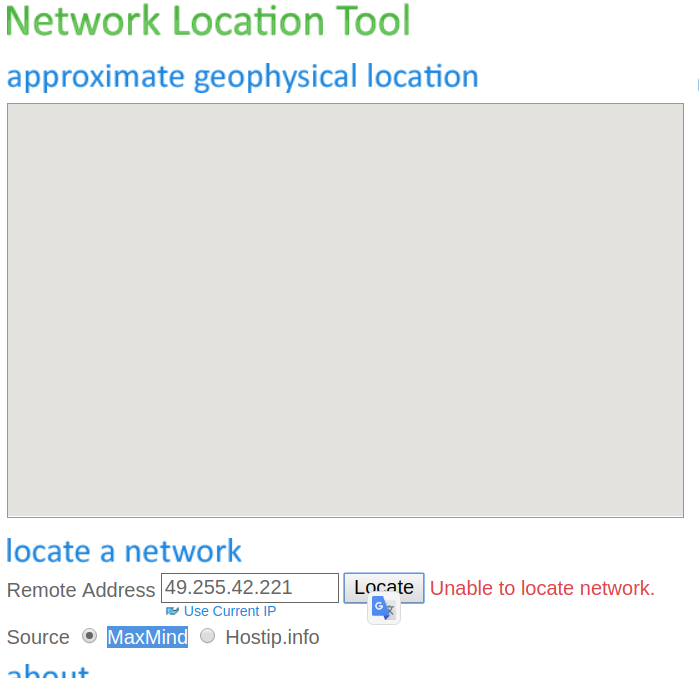
\includegraphics[width=\textwidth]{Location_wont_work2.png}

\subsubsection{Source Data}
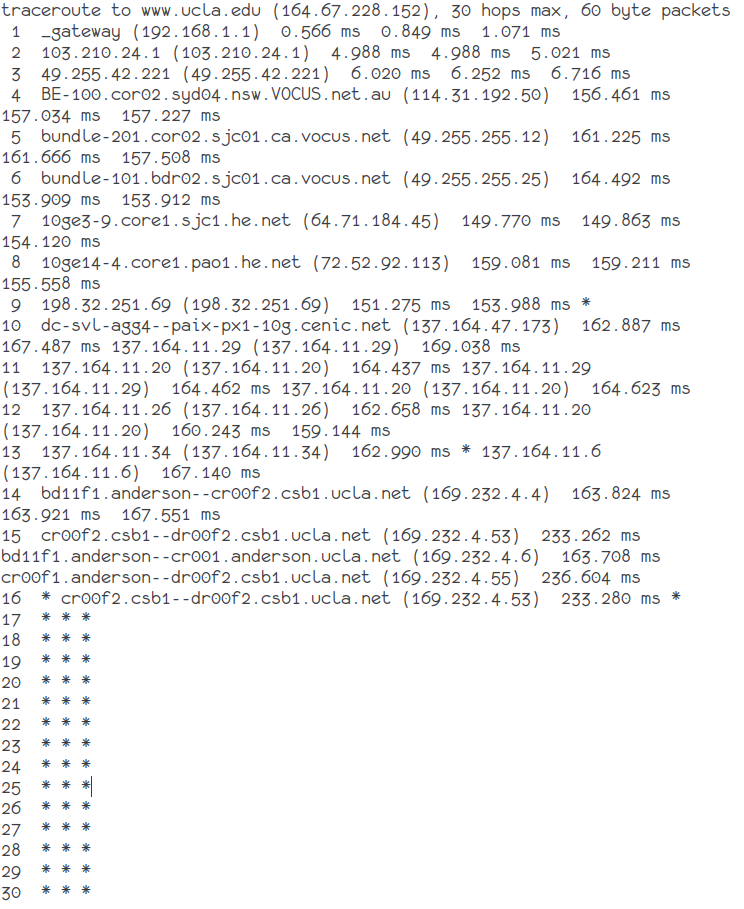
\includegraphics[width=\textwidth]{img/tr_ulca.png}
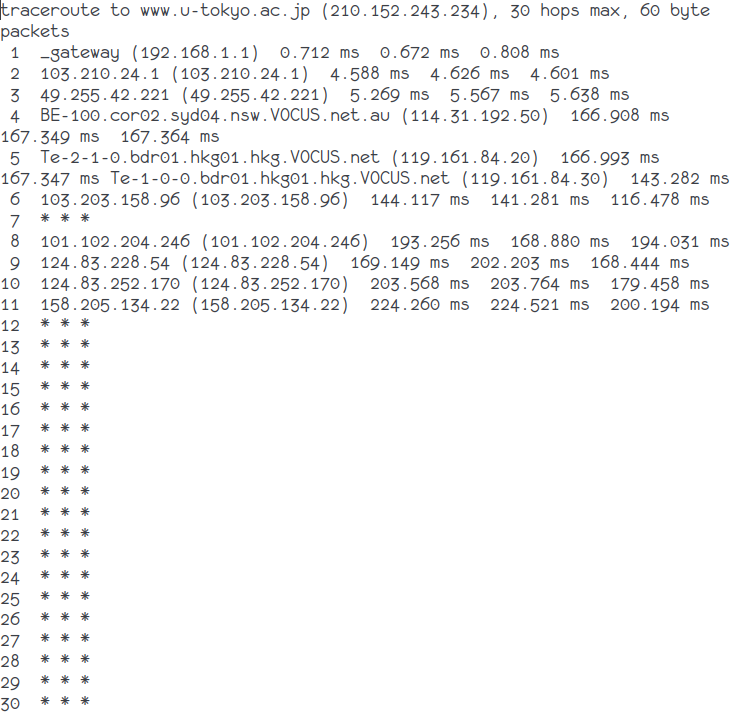
\includegraphics[width=\textwidth]{img/tr_u_tokyo.png}
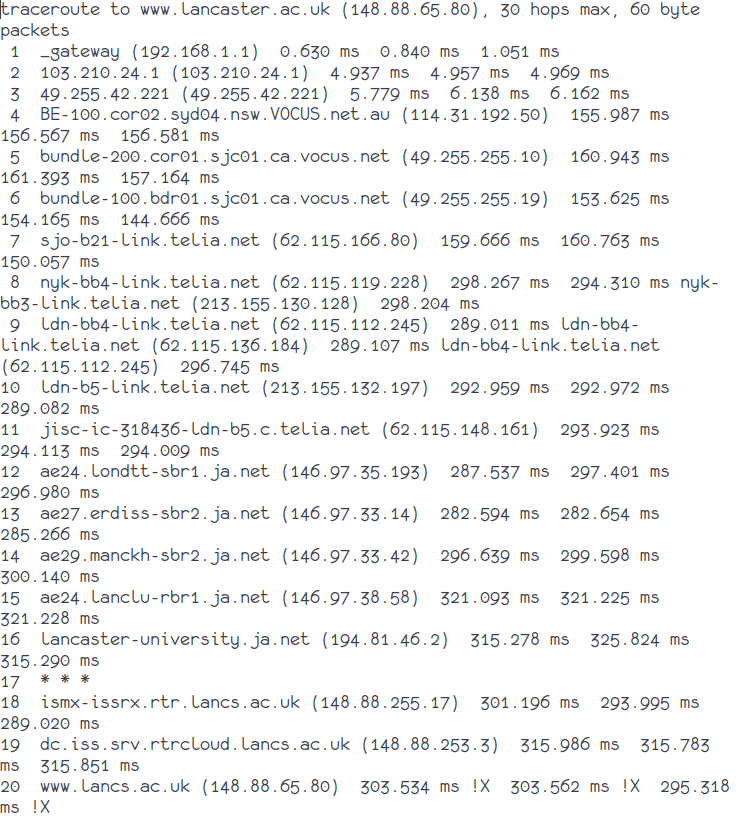
\includegraphics[width=\textwidth]{img/tr_lancaster.png}


\subsection{}
I choose speedtest.com.sg and telstra.net
No, they  didn't go through same  route. I haven't observe any ip is same, but it has a lots of router is belong to vocus. In my opinion, the router have load balancing. Furthermroe, the advantage of package routing is each package can choose the best route when they arrived torouter, which is one of the advantage of package switching. 

\subsubsection{Speed Test Data}
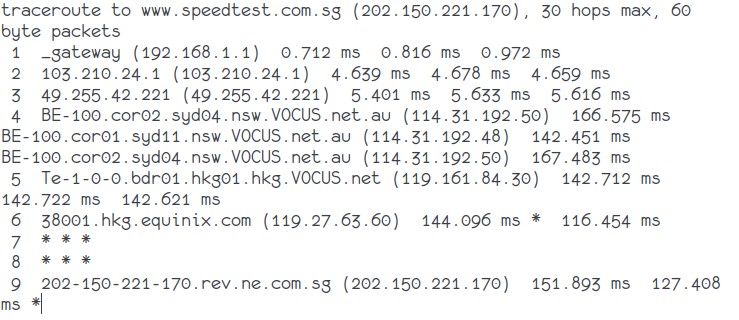
\includegraphics[width=\textwidth]{img/tr_speed_test_host.png}
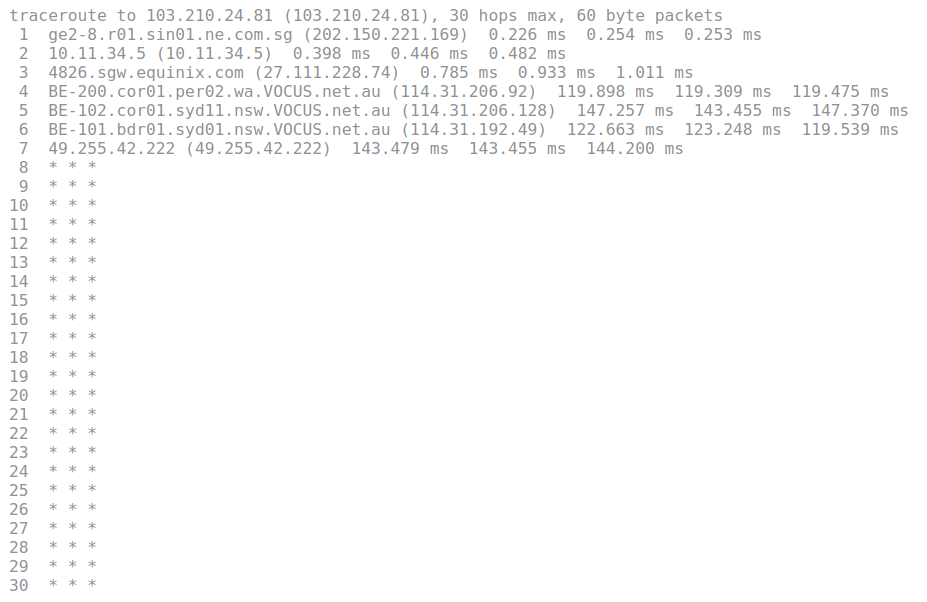
\includegraphics[width=\textwidth]{img/tr_speed_test_dest.png}

\subsubsection{Telstra Data}
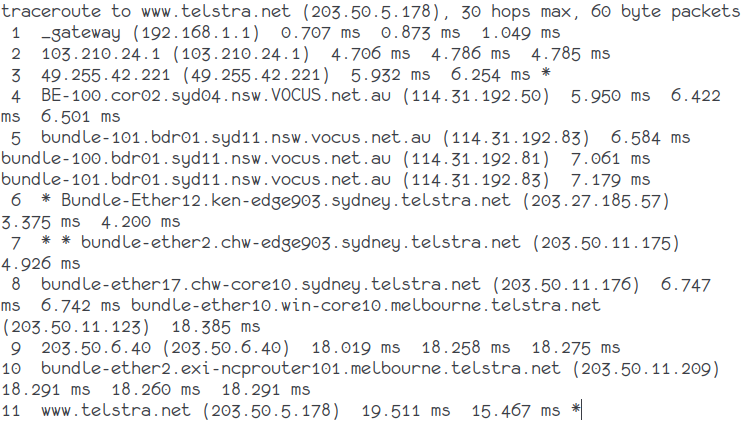
\includegraphics[width=\textwidth]{img/tr_telstra_host.png}
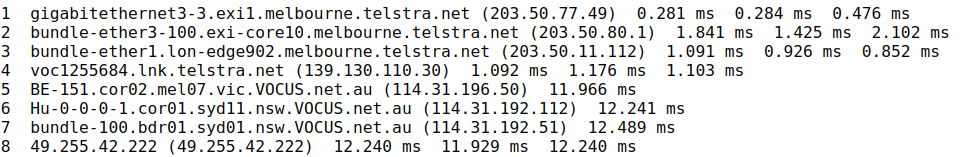
\includegraphics[width=\textwidth]{img/tr_telstra_dest.png}


\section{Exercise 4}

\subsection{Shortest Distance and Time}


\begin{tabular}{|l|r|l|c|}
    \hline
    Hostname & Distance & Time (T) (ms) & Min. Delay\\
    \hline
    uq.edu.au   &   732.13km& 0.002440433&16.669\\
    nus.edu.sg  &  6309.72km& 0.0210324  &142.162\\
    tu-berlin.de& 16076.11km& 0.053587033&307.132\\
    \hline
\end{tabular}

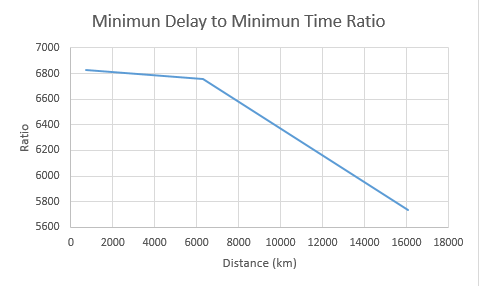
\includegraphics[width=\textwidth]{ratio.png}

\subsubsection{Reasons}
The phisycal wire couldn't be placed at the shortest path. \\
The light or signal in the transfer medium won't neccessary as fast as light (only could be slower than speed of light).\\
The Delay is the sum of \{processing,queueing,transmission,propagation\} dalay, no only the proprogation dalay, and all of the other dalay couldn't be 0.

\subsection{}
It vary over time, because there's a different waiting time (queueing delay) when the package go through a same router each time (because the load of the router is vary). So the sum of all the queueing dalay is vary from time to time.

\subsection{}
\begin{tabular}{|r|l|}
Depend on the package size& transmission delay\\
May depend on the package size& processing, \\
& if the processing is all base on software and has \\
&not accleration from hardware\\
Not depend on package size& {queueing, propagation} dalay\\
\end{tabular}

Further explain, such as checksum, if we all calculated in software, only the O(n) algorithm could be developed, so it will depend on the package size.

\subsection{Graph from This Exercise}
\subsubsection{www.uq.edu.au}
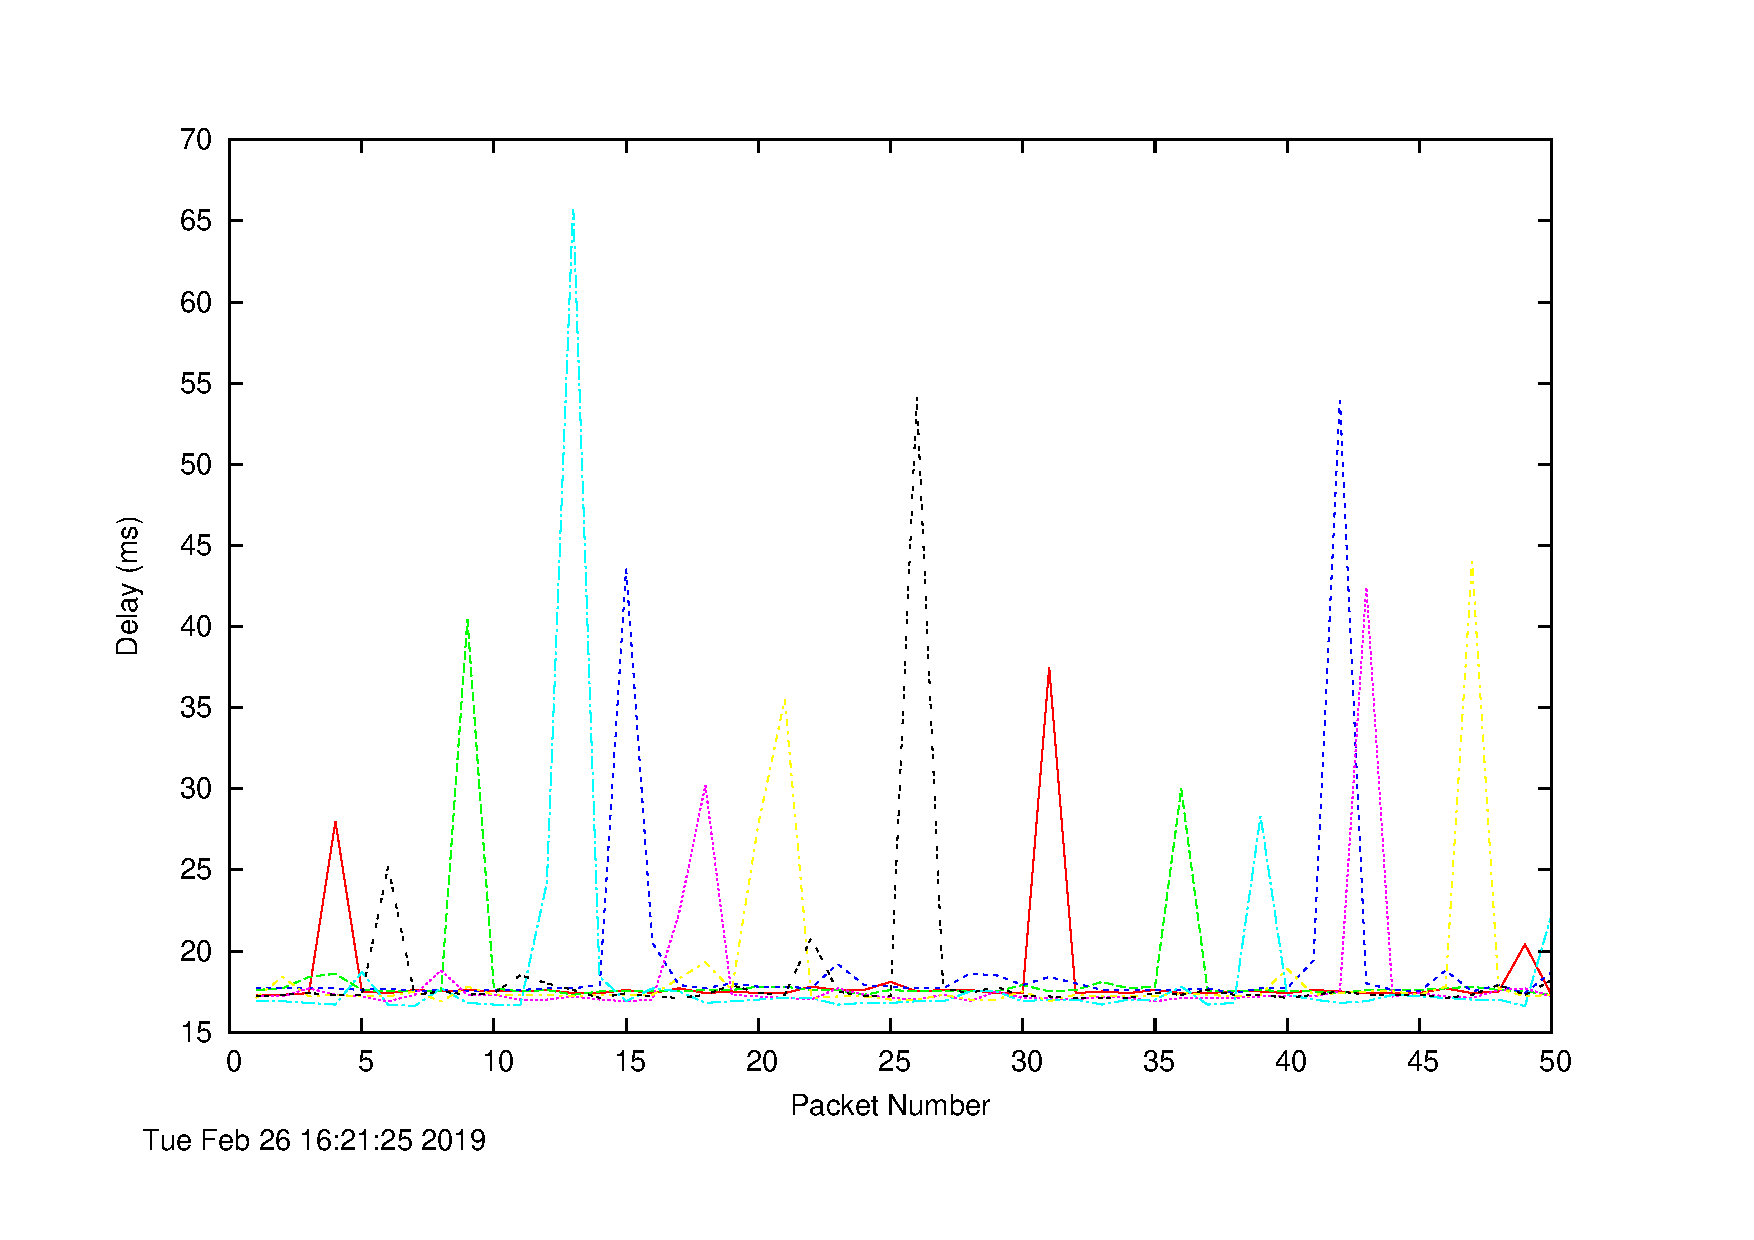
\includegraphics[width=\textwidth]{uq_delay.pdf}
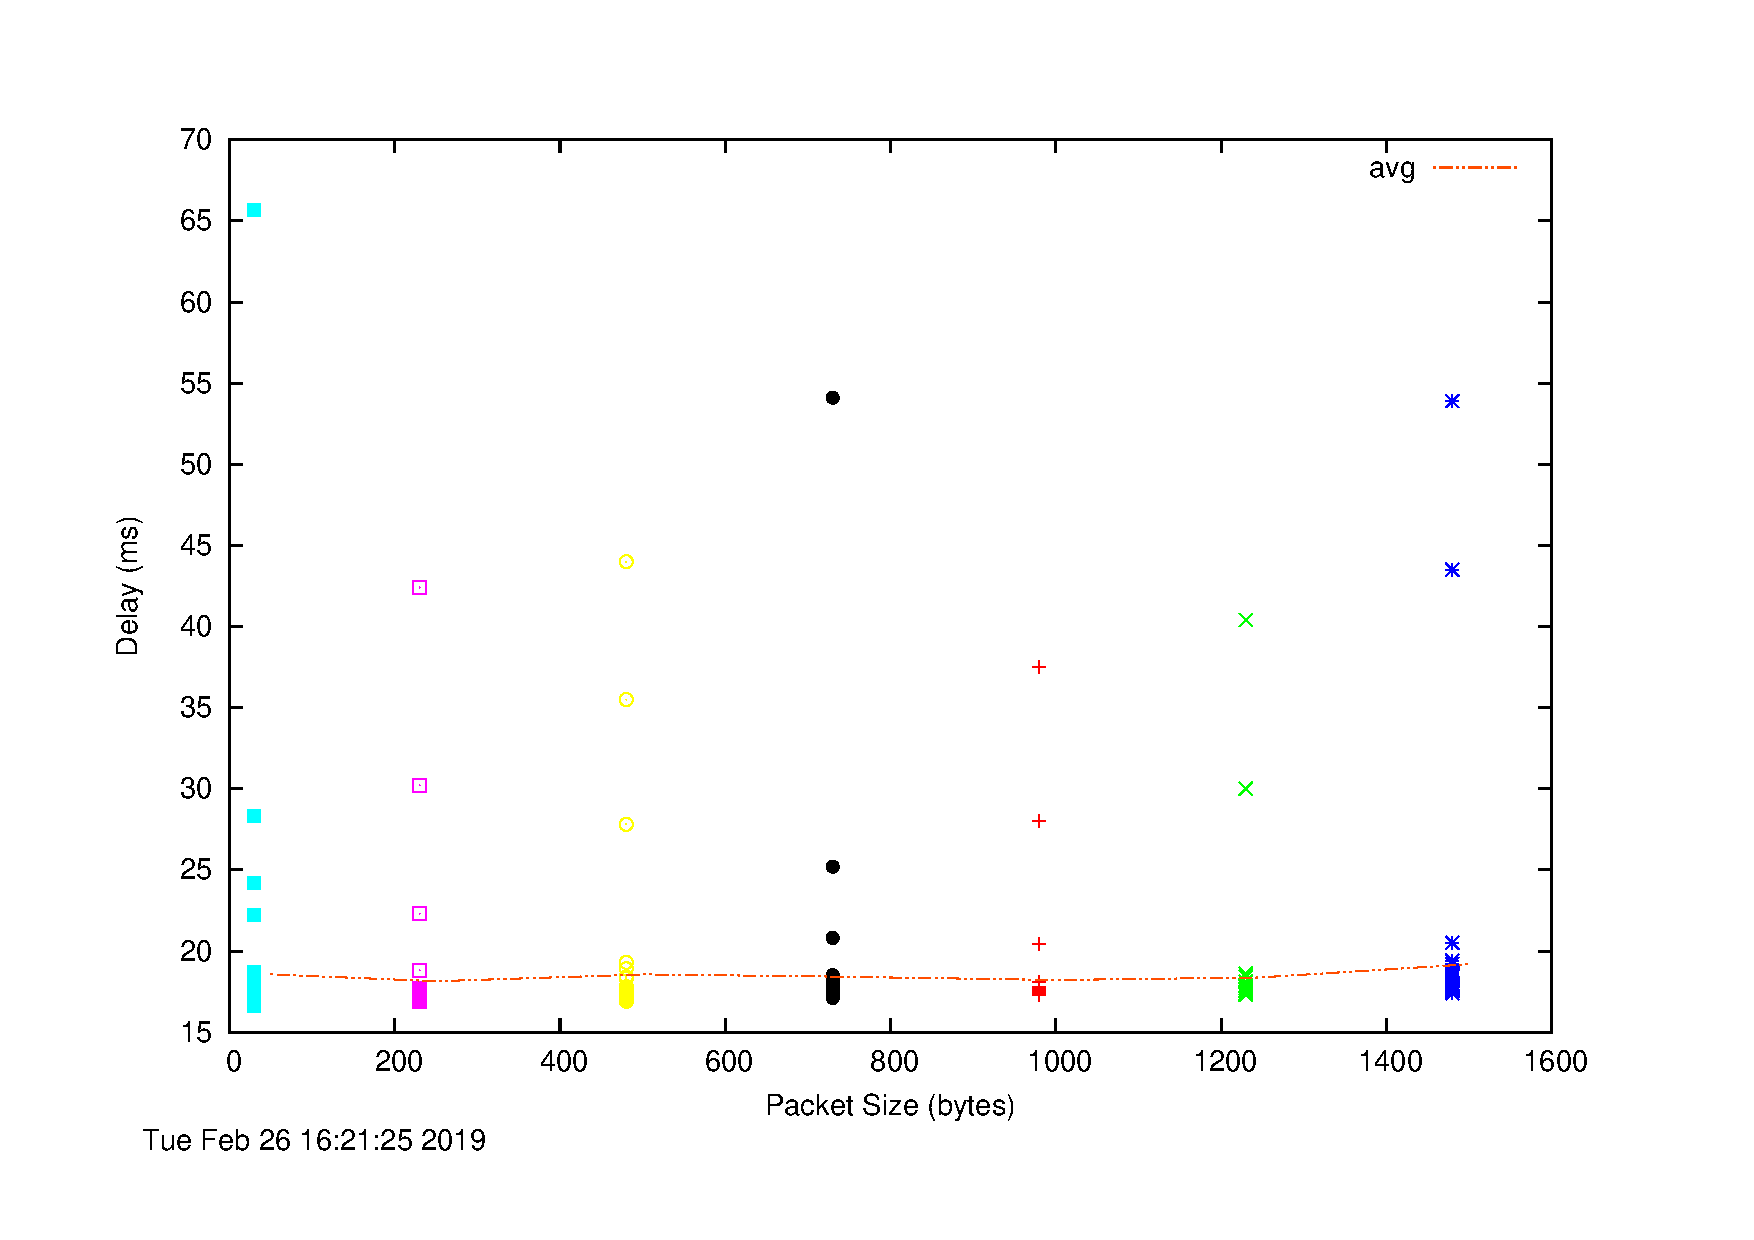
\includegraphics[width=\textwidth]{uq_scatter.pdf}
\subsubsection{www.nus.edu.sg}
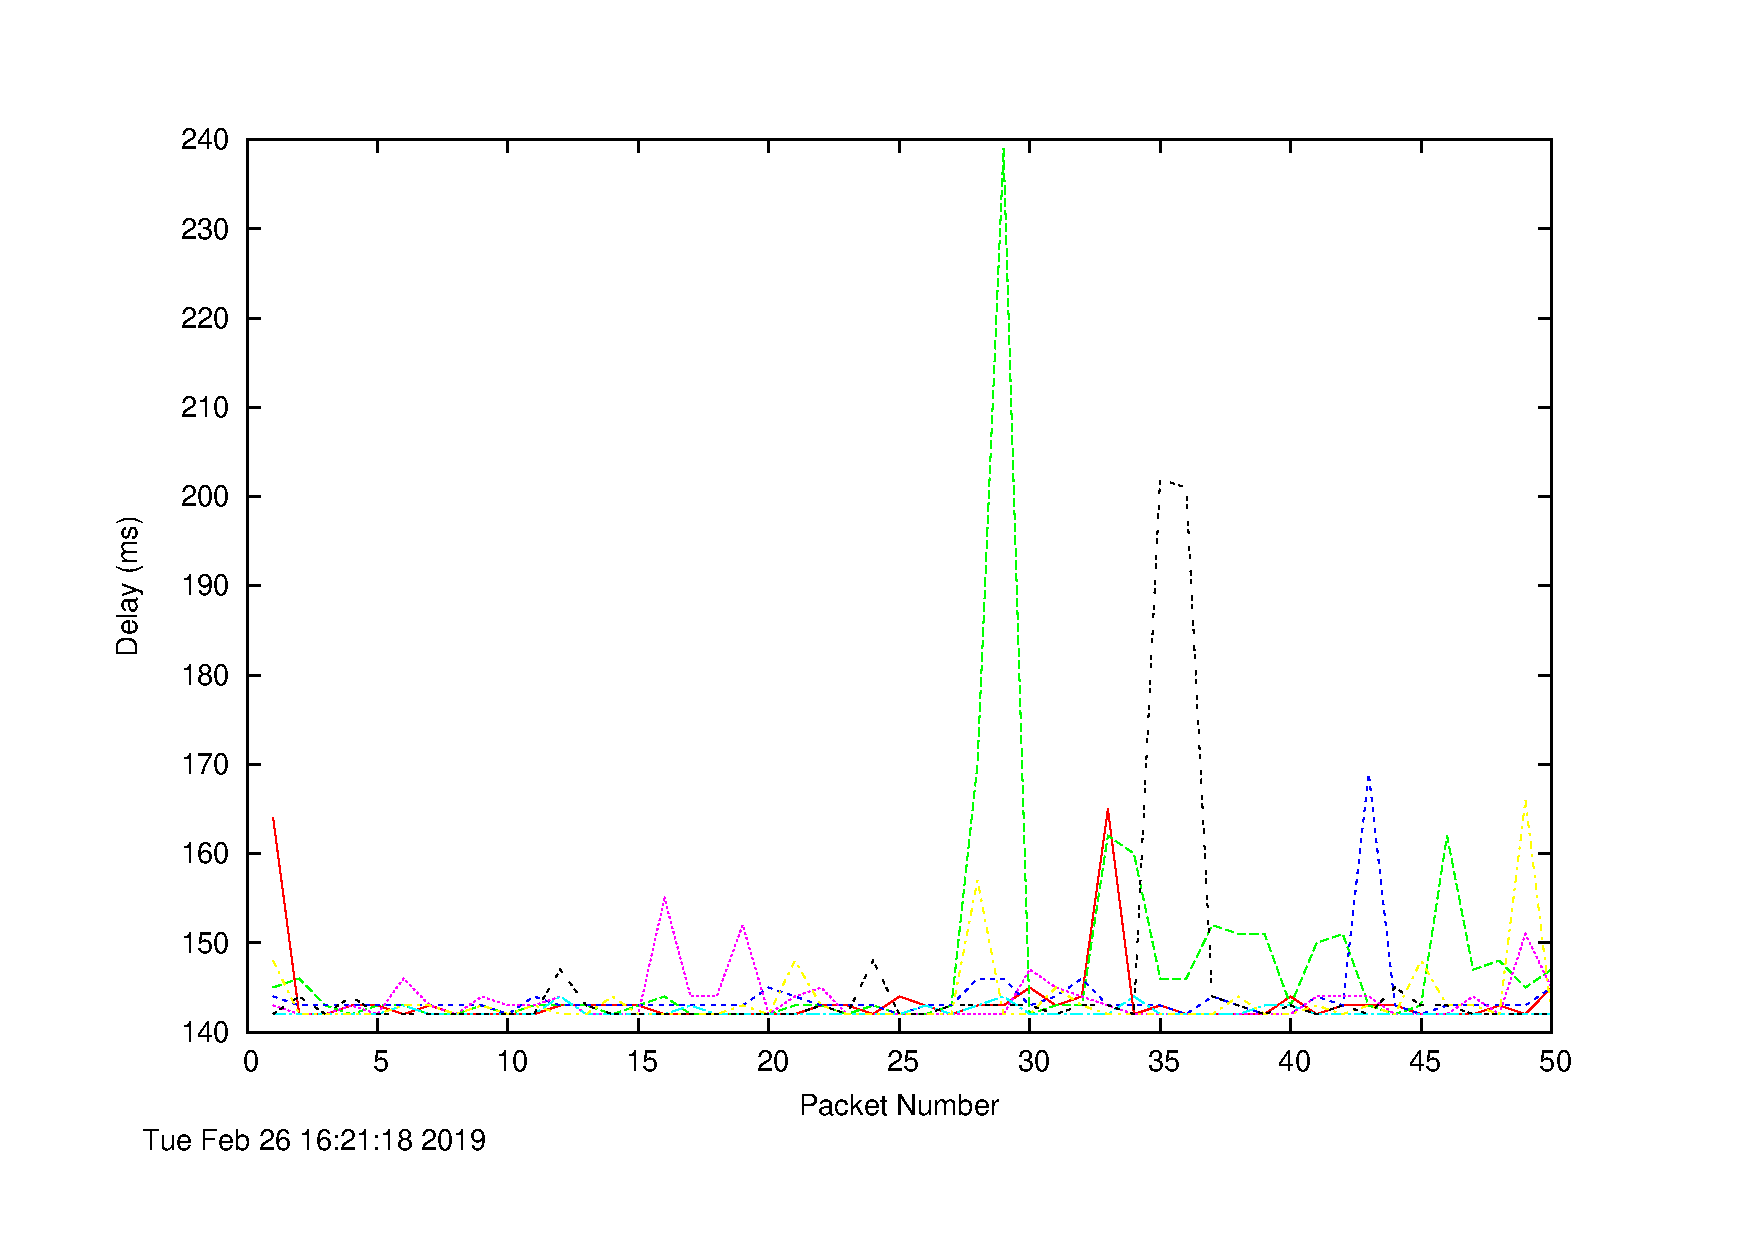
\includegraphics[width=\textwidth]{nus_delay.pdf}
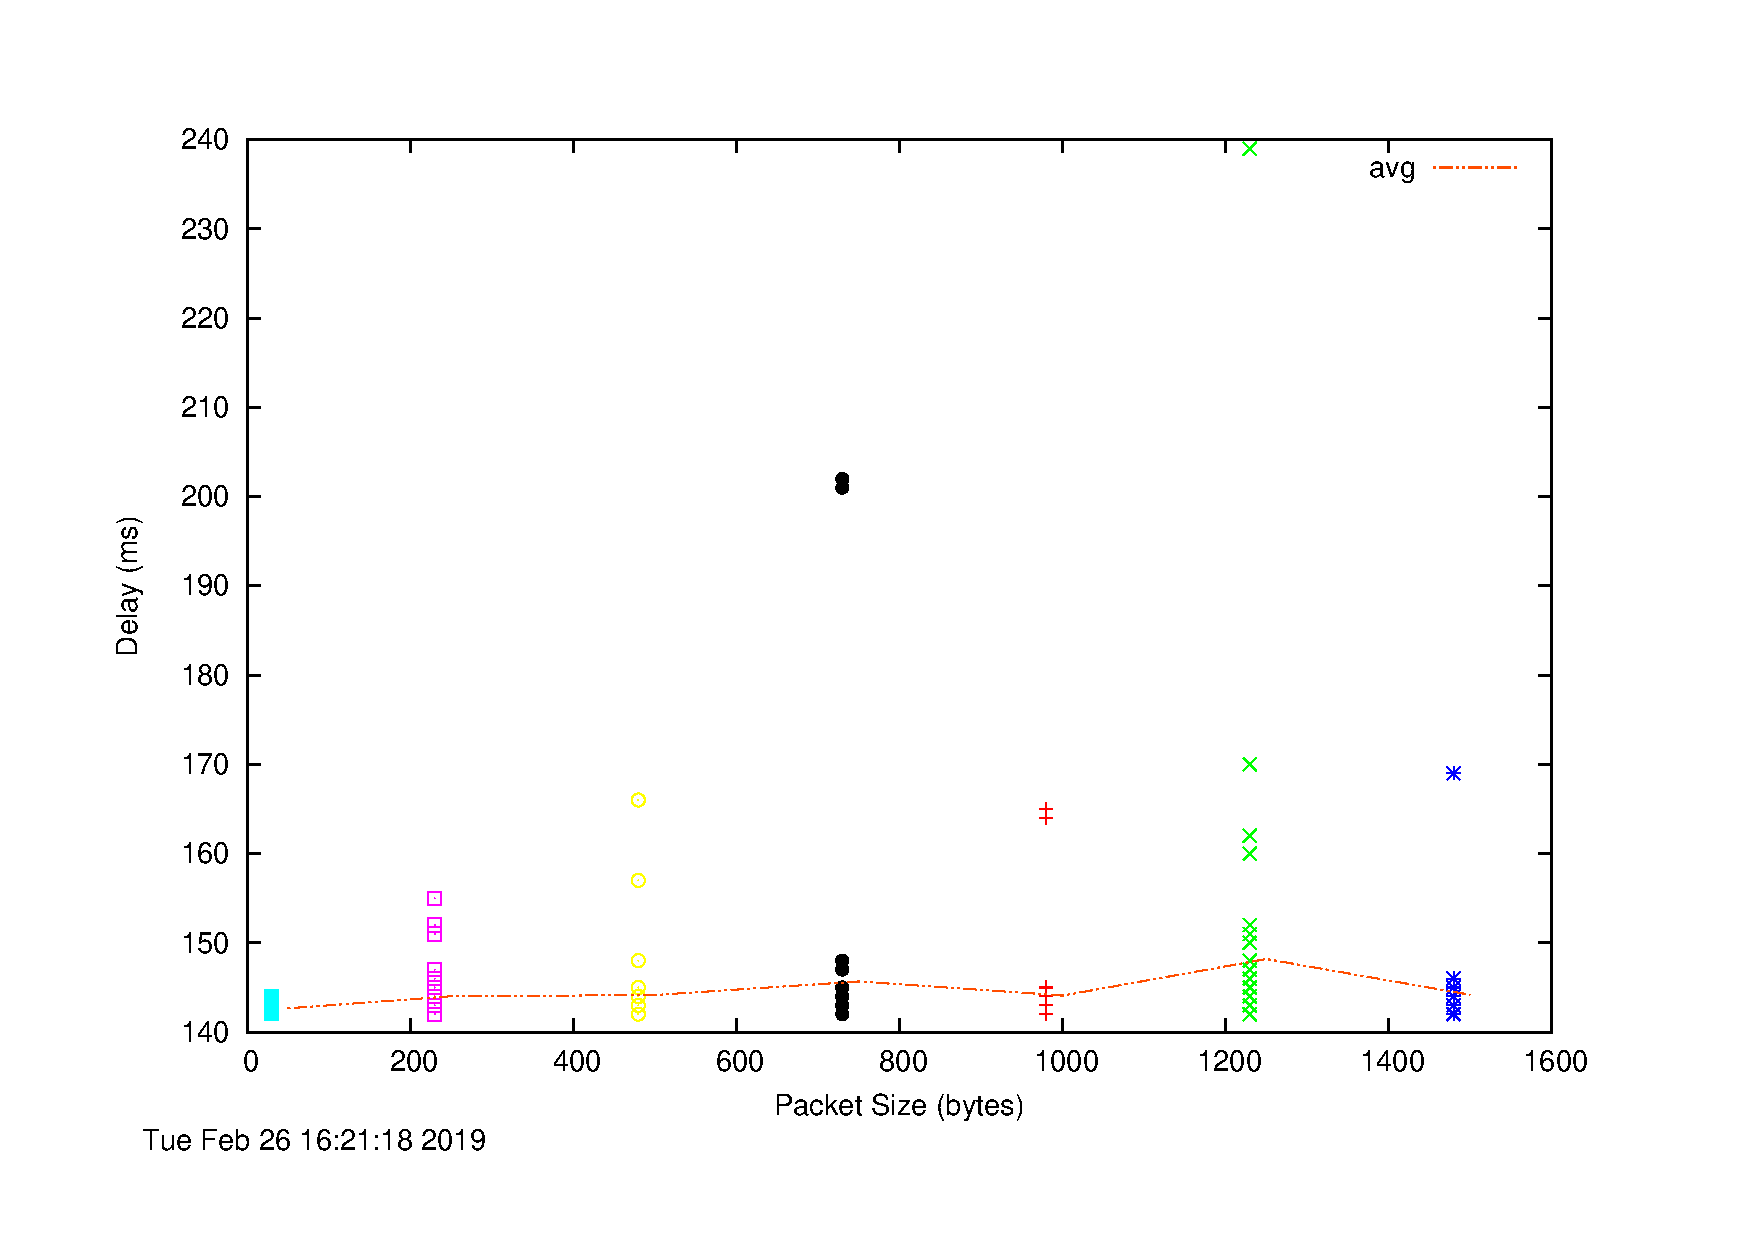
\includegraphics[width=\textwidth]{nus_scatter.pdf}
\subsubsection{www.tu-berlin.de}
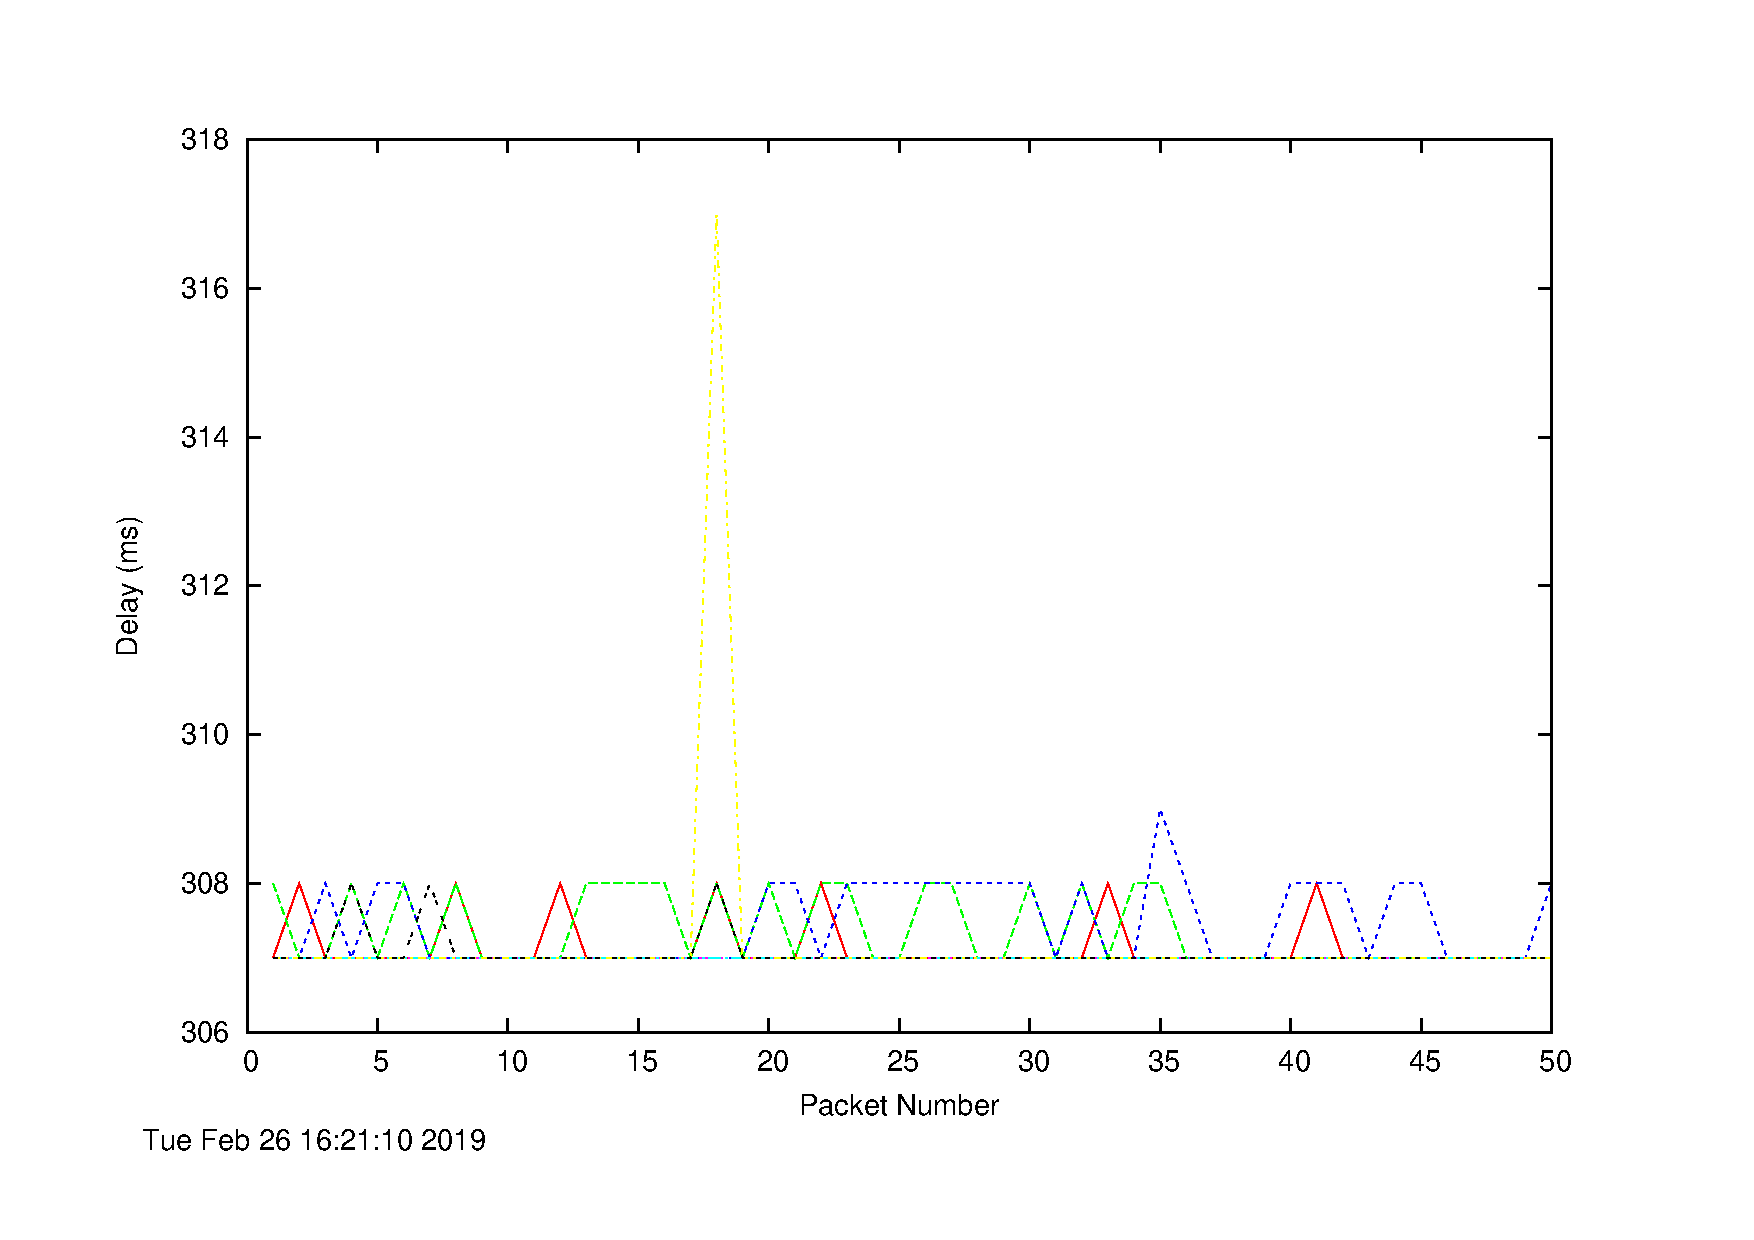
\includegraphics[width=\textwidth]{berlin_delay.pdf}
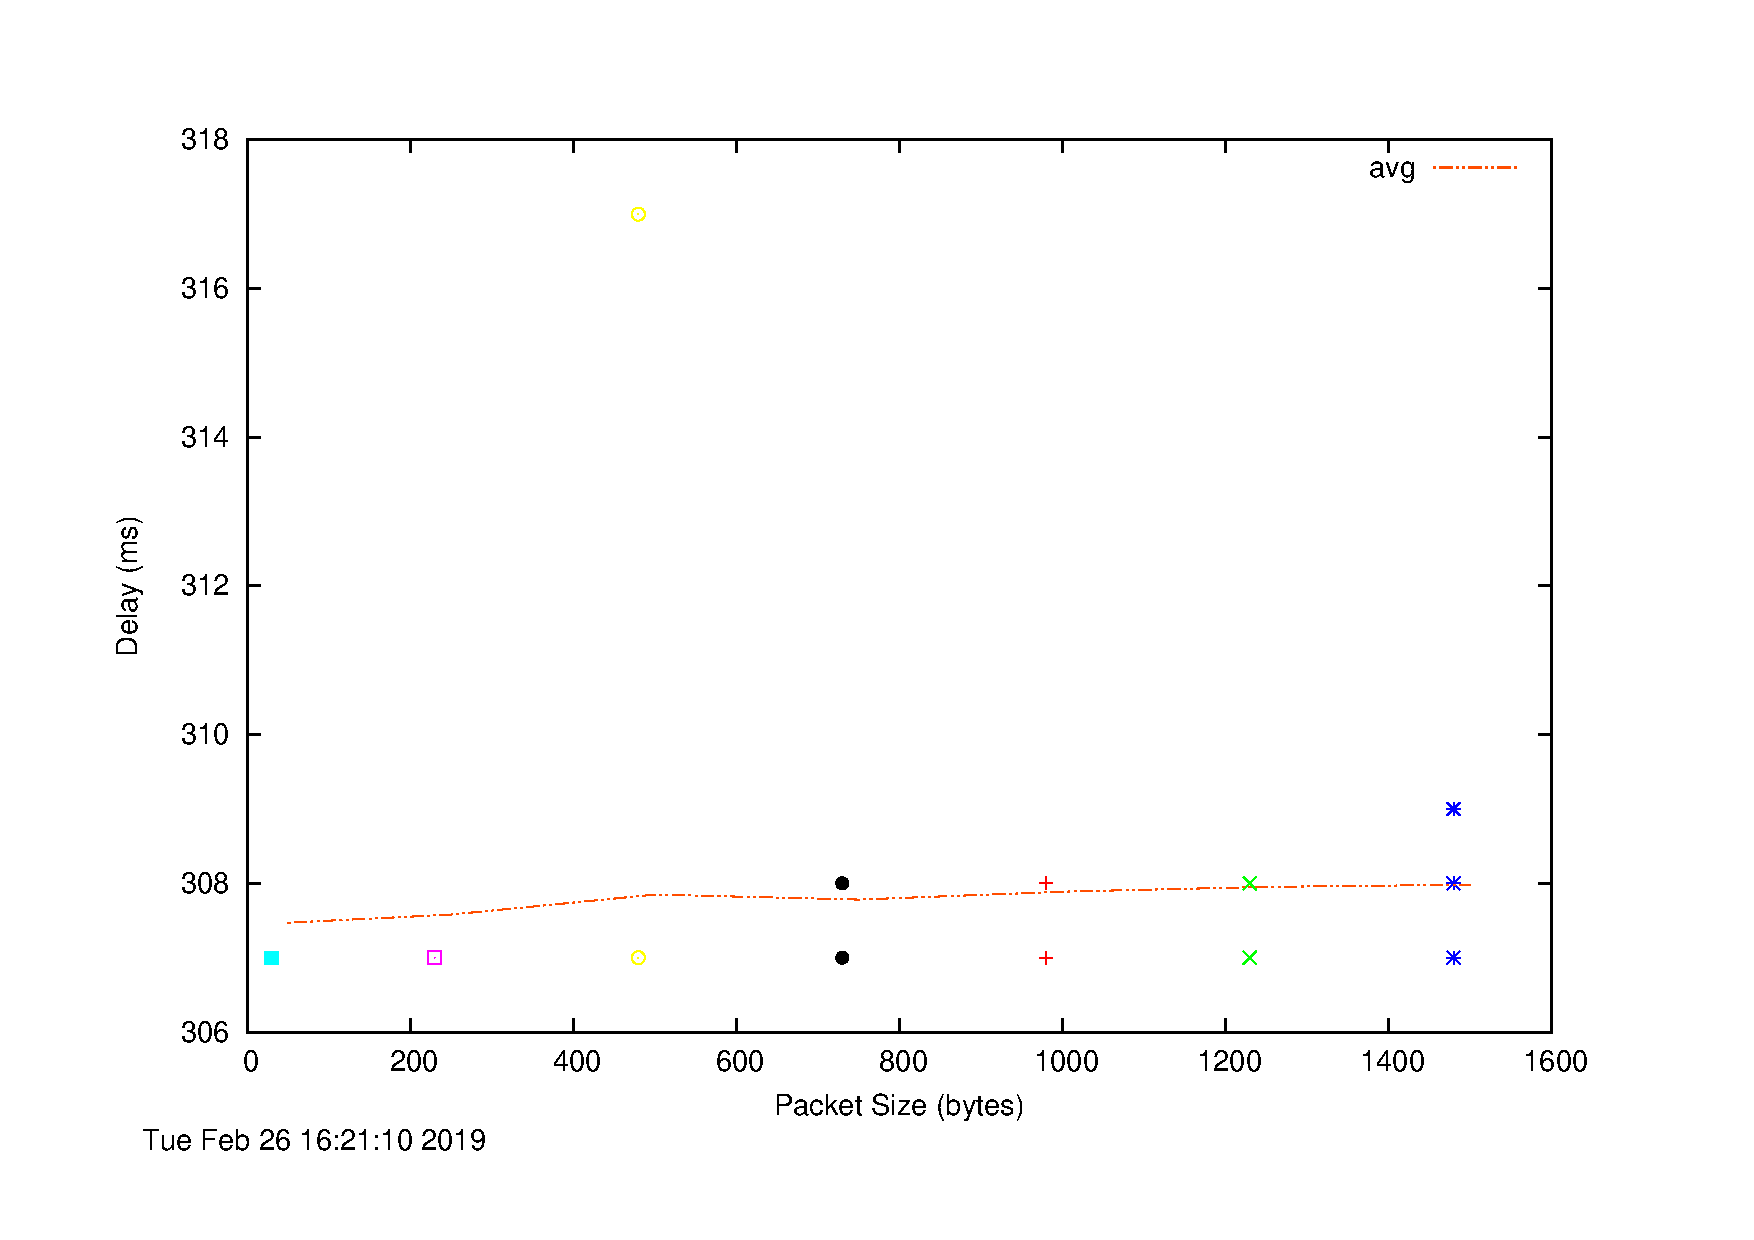
\includegraphics[width=\textwidth]{berlin_scatter.pdf}

\end{document}


